\documentclass[10pt,a4paper]{article}

\usepackage[utf8]{inputenc}
\usepackage[font=small,labelfont=bf]{caption}
\usepackage[english]{babel}
\usepackage{amsmath}
\usepackage{amsfonts}
\usepackage{amssymb}
\usepackage{graphicx}
\usepackage{anysize}
\usepackage{listings}
\usepackage{wrapfig}
\usepackage{attachfile}
\usepackage{hyperref}
\hypersetup{
    colorlinks,
    citecolor=blue,
    filecolor=blue,
    linkcolor=blue,
    urlcolor=blue
}

\marginsize{3.3cm}{2cm}{2cm}{2cm}

\title{MCDRI 1.0 - Multiple Choice Designer, Recognizer and Interpreter}
\date{}

\newcommand{\name}{MCDRI }

\begin{document}

\maketitle
\tableofcontents

\section{Introduction}

\name is a flexible solution for those who regularly use and/or design multiple choice tests. This can be school related tests or exams, questionnaires, psychological tests etc. One of the main reasons to use a multiple choice format is the easiness of scoring them, especially since this task can be automated. Other software in this field has some limitations which we tend to overcome:
\begin{itemize}
\item You are not limited to pre-designed answer sheets as you get complete flexibility over designing your own sheets using a user friendly drag-and-drop interface. You want four questions with nine alternatives, followed by ten true/false questions and finally six questions with four alternatives each? No problem, with a few clicks you'll have designed this and the program will generate an answer sheet in .pdf-format for you to print. Of course some commonly used templates are available too. %TODO: templates
\item \name does not require you to buy answer sheets. Instead you just print or copy the amount needed making multiple choice testing a whole lot cheaper.
\item We do not require you to buy a certain scanner. Nearly any scanner will work (one with a sheetfeeder is recommended). Also keep in mind that nearly every big copier has great scanning capabilities, so chances are high you'll not have to spend any money here.
\item Correcting the tests can be script-based if you want too. This is especially practical if the scoring of your test is rather complicated, like when measuring different scales simultaneously, when different versions are being used, or when the scoring of an item depends on results from other items.
\end{itemize}

Before we go into designing the first, here are some terms we will use often.
\begin{itemize}
\item It may be clear already that the word \emph{test} has a very broad meaning here. Everything containing at least one question can be considered a test, whereby we will only look at those containing multiple choice questions.
\item A \emph{subject} is he or she who fills out a test. So this can be a student, applicant, voter,...
\item An \emph{item} is the combination of a question with one or more alternatives. 
\item An \emph{alternative} is an option that the user can check. 
\end{itemize}

When you open the program you'll see one of the three views in front of you: the Design view. Switching between these views (the others are called ``Import'' and ``Results'') can be done using ``View'' in the menu bar. The following three chapters more or less correspond with these three views.

\begin{figure}
\centering
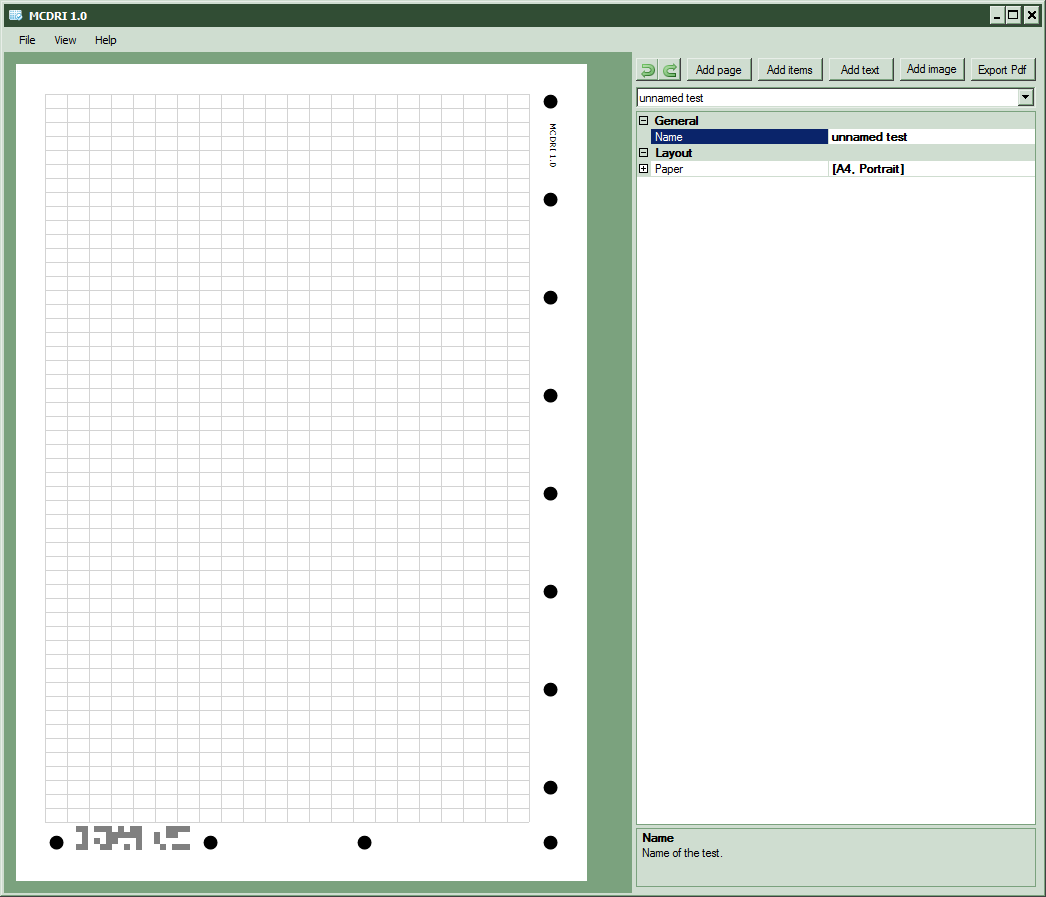
\includegraphics[scale=.55]{img/design.png}
\caption{The Design view}
\end{figure}

\section{Designing a test}

Assuming you are in Design view you have an empty page on the left, some buttons on the right top, and a property pane under the buttons. The design process is similar to programs to make slideshows or web pages by drag-and-drop. You can select anything on the left (currently there only is an empty page), and when selected you can edit it's properties. Click on or next to the the page, and you will see that ``unnamed test'' is highlighted in the property pane. You can change the name of any object with the ``Name'' attribute, for example you can change it in ``my first test''\footnote{If you don't feel like following tutorial-like instructions you can skip all this and find the corresponding file in the examples directory.}. Here you can also set properties of the paper you will use. It is highly recommended to change these settings first as changing them later will mess up your layout. First choose the template: if you are living in North-America you'll probably use ``Letter'', otherwise ``A4'' is the most common format. If you're in doubt what to choose: look at the kind of paper your printer uses. When choosing the paper template, keep in mind that it might be cool to design a test on a 84$\times$120cm A0 paper, but if you don't have the printer and scanner for this you'll not be able to do a lot with that test. It is possible to change the page orientation from portrait to language, but this is probably a less popular format for tests. Another property is the border. Decreasing the border size this will give you a slightly bigger design zone, but there is a risk that your printer will not handle this correctly, so it's recommended to leave the default value. There also is a property called ``Blocks'' which you can't change. This describes the remaining space after setting the paper template and the size of the border.

Now take a look at the page on the left. The grid you see correspond with the number of blocks. This grid will not be printed but makes it easier to align the different elements we're going to add to the page(s). The black rounds on the right and bottom of the page are used for alignment. On the bottom right is a matrix bar code which is used to determine if the right test is used to correct scanned pages and also contains the number of the page. 

The buttons on the top right are undo/redo, some buttons to add elements to your test, and the export button which we will discuss later. Most options are also accessible by right clicking on a page. There are three kinds of elements you can add to your test:
\begin{itemize}
\item Itemset: this is the core of your test. Itemsets can contain questions, identify which version of the test the subject filled out, and identify the subject.
\item Text: this can be used to add some extra information or instructions to your page.
\item Image: to add a logo of the school or company etc. All common graphic formats are supported.
\end{itemize}

All elements have properties for location (Grid position; co\"ordinates measured from the top left of the page) and size which you can change in the property pane. The location can also be changed by dragging an element. Size cannot be set manually for itemsets, but more about that later. Make sure all elements are placed within the grid, otherwise you'll not be able to create a .pdf-file. You can also choose if you want to have a border drawn around your element or not.

\begin{wrapfigure}{R}[0cm]{0.45\textwidth}
\centering
\vspace{-10pt}
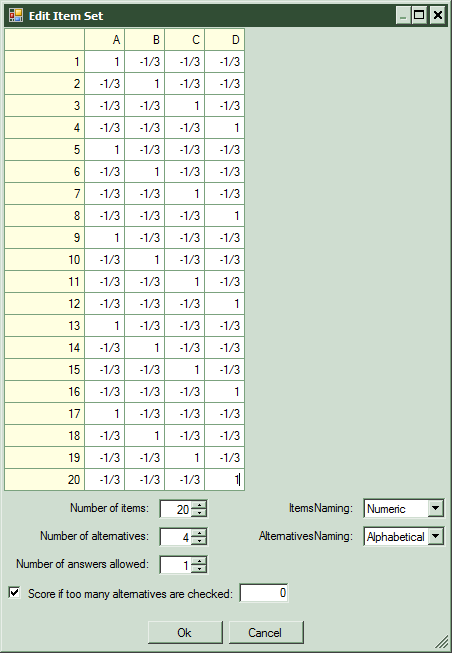
\includegraphics[scale=.55]{img/edititemset.png}
\caption{Setting score values for the questions}
\vspace{-25pt}
\label{fig:settingscores}
\end{wrapfigure}

You can add also add other pages and move test elements from one page to another, but in most cases your test will probably fit on a single page. 

Now we will go into more detail using a simplistic example of an exam:

\subsection*{Itemsets: the core of the test}

We will need two itemsets, one for identification and one for the questions.

Let's assume we have twenty questions with four alternatives each. As all these questions therefore have the same format we can use a single itemset. Add an itemset to the page, change the name and description properties both to ``Answers'', and the role to ``Question''. Change the number of items to 20, the number of columns to 2 and the number of alternatives to 4. Double click the itemset to set the points a subject receives for certain answers. For easiness of the example we will use the order A B C D A ... as correct answers. Every correct cell needs the value for correct (1), and every incorrect cell needs the value for incorrect (-1/3 in this case). To make it easy, use your mouse to select all cells from A1 to D20, right click, and choose ``Set multiple weights''. In the textbox in the dialog set the value to -1/3 and press Ok. Now we only have to change the cells corresponding with correct answers to 1 like in Figure \ref{fig:settingscores}. These are A1, B2, C3, D4, A5 etc, which is of course not smart for a real test but it keeps it clear in this example. Finally, set grid position to 6;34. You might have noticed that the size of the itemset automatically changes when you change the number of items, alternatives, columns etc.

For the identification, add another itemset. Change the name property to ``ID'', the description to ``Identification'', and role to ``Identification''. We assume that every students ID in this example exists of eight numbers, so change the number of items to 8 and the number of alternatives to 10. Change the number of columns to 2 as this will fit better. The names of items and alternatives are wrong however: as can be seen in the instructions the items need to be called A, B, ... while the alternatives should be a number from 0 to 9. The item names can easily be changed by changing the ``Items naming'' property to Alphabetical. For the names of the alternatives we can not use the build in Numeric naming as this starts with one, not zero. Double click the itemset and manually change the top row from A-J to 0-9. You can even write text in the row- or columnheaders (names of alternatives or items respectively), but this does not add up to the clarity of your answer sheet\footnote{An example where this would however be useful is when measuring opinions on a scale from for example ``Strongly disagree'' to ``Strongly agree''. If your questions are also very short you can even change the itemnaming to your questions so you won't need a separate answer sheet.}. You do not need to change the zeros in the datagrid like we did with the questions as identification doesn't have right or wrong answers. Finally, set grid position to 0;26.

If you would use multiple pages and you are correcting multiple subjects simultaneously you'll have to add an identification itemset on each page (using the copy/paste functions you'll find under right mouse menu will help you with that).

\subsection*{The text element (and some notes on instructions)}

A text element is used for additional explanations not fitting in the description of an itemset. To change the text, click on the right of the ``Text'' property field. A bigger field will appear making it easier to enter larger amounts of text. To start a new line use Ctrl+Enter. In case of larger texts it might be practical to prepare them in a text editor.

Add a text element to the page, set the grid position to 0;4 and the size to 22;21, and paste the content of \textattachfile[color=0 0 1]{examples/my first test/instructions.txt}{this file}\footnote{In case you're reading this on paper or can't open the link for another reason: The file ``instructions.txt'' that comes with this example contains the same content.} in the ``Text'' field of the property pane.

The amount of instructions in this example takes up a lot of space, but as we only have a limited number of questions one page is still more than enough. However, if you would need more space we recommend to place the instructions on your questions sheets. The same goes for the questions themselves: technically you could put them on the answer sheet but you'll most likely result in a loss of clarity.

\begin{wrapfigure}{R}{0.4\textwidth}
\centering
\vspace{-25pt}
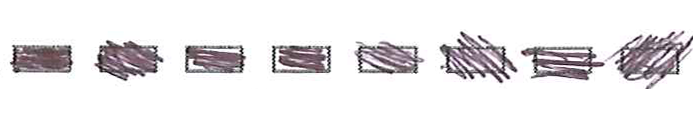
\includegraphics[scale=1]{other/good.png}\\

\includegraphics[scale=1]{other/bad.png}
\caption{``Good'' (top) versus ``Bad'' (bottom) ways of filling out the boxes.}
\vspace{-5pt}
\label{fig:goodbad}
\end{wrapfigure}

Good instructions are vital if you want to receive good filled out sheets that are corrected without a glitch. We recommend you not to rely on written instructions only but also explain it verbally. For those using this for exams: we've seen a great gain in organizing a dummy exam that students could voluntarily attend. Not only were students better prepared for the real exam as they were already used to the system, it also gave us the opportunity to adjust the instructions where necessary. Don't forget to tell the subjects what are good ways to fill out the boxes. If the boxes are just ticked instead of filled they will be considered to be doubtful cases by the software which will result in extra work for you when correcting as you will have to set the value manually. On the other hand subjects tend to be overly careful (and thus loosing time which might be critical in case of an exam) when they now an answer sheet is corrected by a computer, while in reality the system is certainly smart and flexible enough. In the case of an exam you can use a projector to show good versus bad filled out boxes, or if you have some place left on the answer sheet you can add the corresponding images like Figure \ref{fig:goodbad} which you can find in the ``other'' directory.


\subsection*{The image element}

Add an image element to the page and set the image to ``logo.png'' which you can find in the example directory ``my first test''. Set the grid position to 6;0 and the size to 10;3. Set the border property to false. For the other options the default values are just fine.


\subsection*{Saving, exporting and printing}

Don't forget to save your test using ``File'' from the menu bar. If you're not sure you've got everything done right you can open the test from the examples directory. Click ``Export Pdf'' in the right top to generate a printable version of the test. If you're using an unlicensed version of the software a watermark will appear on the file; this is of course not the case if you have a licensed version. A4 paper is used in this example, but you can print this on Letter-size paper without problems.

Some printing tips:
\begin{itemize}
\item If gray levels are handled correctly, the rounds on the side and bottom should be pitch black, while the matrix bar code has to be gray. If the bar code is printed completely in black, then importing and interpreting will be harder. You can set the gray level of the barcode as a property of the test (just click on a page in Design view) if your printer does not handle it correctly. 
\item Gray levels are not a problem on inkjet printers, but on laser printers some tuning might be required. If you're using a laser printer look for a setting called ``Halftoning''. Higher values (e.g. $9\times9$ instead of $3\times3$) generally generate more reliable levels of gray.
\item When you think you've found the right printer settings, test a page (as we will explain in the following section). You don't want to end up doing a lot of extra work because a bad printed page results in difficult to interpret scans.
\end{itemize}


\section{Scanning, importing and optical mark recognition}


This are the minimum scanning settings you should use. These settings are in reach of every scanner.
\begin{itemize}
\item You have to use at least 8 bpp (bits per pixel) gray scale. Pure black-and-white, also called monochrome, monotone or 1 bpp will not work. Color is ignored, so scanning in color unnecessarily increases the file size.
\item Set the scanning resolution at 300 dpi (dots per inch). Perfect accuracy can be obtained at this level of detail, and using a higher dpi will unnecessarily increase the file size and the time the scanner needs to compress and send the file (especially with cheaper models this often forms a bottleneck).
\item The fastest scanners in general are big copiers. Apart from the option to email scanned images, which is only practical if the number of pages is small due to limitations in email boxes, they (nearly) all have the capability to scan directly to a network disk or a folder on your computer.
\item Taking photographs of the test will not work.
\item Do not use a hand-held document scanner.
\item Avoid using lossy compression (like JPEG) in your scanner settings. Either use lossless compression (like PNG) or no compression at all. If you do need to use lossy compression, then use the highest value for quality available (i.e. the least amount of compression).
\item Rotated or upside down pages are not a problem for \name to recognize but it will take a lot more time, so try to put every page right size up in the scanner.
\item To make sure you'll get the best results (i.e. the least amount of manual work left), do a calibration procedure before you start. You can find this option in the right top corner of the ``Import'' view. You need an scan of an empty test for this. Due to differences in paper, printers and scanners that you can use this is necessary.
\item A lot of scanners provide the scanned images in pdf-format which cannot be read by the current version of \name. A simple solution to this problem is installing Ghostscript (freely available) and running a batch script like this:
\begin{verbatim}
@echo off
echo This may take a while...
pushd "C:\Program Files (x86)\gs\gs9.09\bin"
gswin32c -sDEVICE=pngalpha -r150 -o^
         "C:\Users\...\scan-%%d.png"^
         "C:\Users\...\scan.pdf"
echo.
pause
\end{verbatim}
\end{itemize}

Now let's imagine someone filled out the test we just designed. Open the test ``my first test.test'', and go to the ``Import'' view. Click the ``Import'' button to add the file ``my first test.png''. We only have one page now but normally you would of course import a lot of files at the same time. In the licensed version of \name there is no hard limit to the number of files you can import simultaneously, so it's up to the amount of RAM in your system. As a rule of thumb, 1000 pages in A4 or Letter format take up about 2 Gb of RAM.

On the left you can see the scanned page corresponding with the selected file in the datagrid on the right (but there currently only is one). The slider on the left top op the image lets you zoom in or out. You can use the mouse with the left button pressed or the scroll bars to drag the scanned image. 

On the right there is a datagrid showing all the imported images. Following the file name is a question mark because the page number is not yet known as the image is not yet analyzed. Following are six positions for icons to appear that give information about the status of the scanned images. The following table gives an explanation for all possible icons:\\

\begin{tabular}{l|p{.8\textwidth}}
Icon & Meaning \\
\hline

\includegraphics{img/icons/NotAnalyzed.png} & \vspace{-20pt} The image has not yet been analyzed. \\

\includegraphics{img/icons/ContainsDoubts.png} & \vspace{-20pt} There are cases of doubt: for certain boxes it is not clear whether they are checked or not. These are shown in red. If you have a lot of these calibration is required.\\

\includegraphics{img/icons/ContainsTooManyChecked.png} & \vspace{-20pt} More boxes are checked than acceptable. Usually this happens when the subject ticked too many alternatives for one item or when he or she has corrected an answer. If you see \name thinks certain boxes are checked while they are not, calibration is defiantly required.\\

\includegraphics{img/icons/BarCodeError.png} & \vspace{-20pt} The bar code could not be read. Check if the scanned page corresponds with the test, and if that is the case right click on that row and choose ``Set page number''.\\

\includegraphics{img/icons/PageNumberOrHashError.png} & \vspace{-20pt}  The bar code does not fit the open test. Check if the scanned page corresponds with the test, and if that is the case the bar code might be damaged; right click on that row and choose ``Set page number''.\\
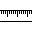
\includegraphics{img/icons/CalibrationError.png} & \vspace{-20pt} \name tried very hard but really couldn't recognize this image as a test page. If this has happened to multiple files then the problem is likely with the scan settings. If it is only a single case this might be a result of a ``damaged'' sheet (folded, writings near the black rounds, ...) in which case you'll have to remove this from the datagrid and correct it manually. The last possibility is of course that it wasn't a test sheet at all that ended up between your sheets. \\
\end{tabular}\\[10pt]

You can sort the columns of the datagrid by clicking on ``File'', ``Page'', or one of the buttons marked with a caret. This is especially practical when you have a lot of scanned images and only want to go over those that show a certain error. Press ``Analyze all'' to start the optical mark recognition process. For a single page this won't take long, but keep in mind this can take a while if you're analyzing a big pile simultaneously. When this process fails for a certain page, \name will try again with slightly different settings and repeat this process until a solution is found or until it runs out of options. This means that ``bad'' pages will slow down the total process a lot, therefore make sure you have no other pieces of paper in your scanned pile. When you do have a lot of scanned pages it's also highly recommended to first only analyze a few to see if everything is working fine. You can do this by selecting a few rows in the datagrid and choose ``Analyze'' via the right mouse button menu. Optical mark recognition is a very heavy process for the CPU. \name is highly optimized to do this process as quick as possible, but still the actual speed will depend on the kind of processor in your system. Both raw CPU-speed as the number of cores are of importance for the performance as \name works multithreaded. It's difficult to give an estimation of how long it will take due to the large number of contributing factors involved, but if you're analyzing hundreds of pages simultaneously we advice you to go get a cup of coffee while doing so. 

\begin{wrapfigure}{R}[0cm]{0.45\textwidth}
\centering
\vspace{-10pt}
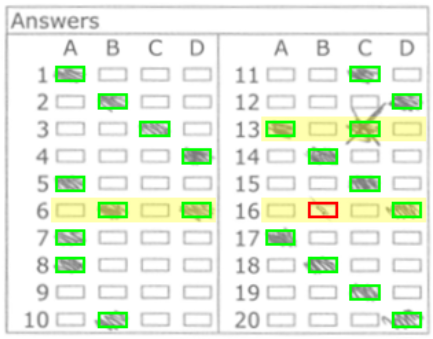
\includegraphics[scale=.55]{img/impfirst.png}
\caption{In this example some manual intervention is necessary.}
\vspace{-0pt}
\label{fig:manualintervention}
\end{wrapfigure}

If you analyze the filled out and scanned page ``my first test.png''. You see that the identification itemset is filled out well but that there are some problems with the answers itemset like you can see in Figure \ref{fig:manualintervention}. Of course the goals is to have as little manual work as possible, which will be obtained by giving the subject clear instructions. However occasionally you'll have some extra work like in this (deliberately bad) example. On item 6 the subject has ticked two boxes while the instructions were clear that only one answer is allowed per item. You can either set both to ``Unchecked'' using the right mouse button menu on the box, or you can leave it in this case as we use the default setting is to give a score of zero in the case of too many checked alternatives (See Figure \ref{fig:settingscores} at the bottom). If you use the latter option, the error will however remain to be shown. We see a similar problem with item 13, however this seems to be a correction. Let's assume that the subject first checked alternative C but then changed his or her mind, scratched C, and choose A. We therefore set the status of box C to ``Unchecked''. It is of course up to you how to handle this kind of situations. You can also give the instruction never to correct but this will result in a lot subjects having to start over again on a new sheet. Certainly on time critical tests like most exams this is not a good idea. We suggest to allow subjects to correct a few mistakes (make clear in advance how corrections should be made!), but to ask for a new answer sheet if it becomes too messy. Finally, there is a problem with item 16. It seems to be clear that the subject choose alternative D, so we leave that one checked, however there is a rectangle at alternative B, indicating a case of ``doubt'': \name doesn't know for sure if the box is checked or not. In this case it seems to be an unintentional scratch, so we set this box to ``Unchecked''. As we solved all three problems you'll see that the corresponding error items in the datagrid have disappeared. 


\section{Interpreting the results}

Go to the ``Results'' view. There is a new datagrid with one line for each subject. In the itemset where role was set to ``Idendification'' the subject answered 12345678 which can be seen in the first column. If no identification itemset was present the file name will be put there. After a column with the number pages there is a column ``Total'' which shows the sum of all itemsets with their role set to ``Question'', so Identification and Version itemsets are ignored for the total score. Then for each of these itemsets there is a separate total score (identical value to the test total here of course as there is only one), optionally followed by separate scores for each item in that itemset (there are three checkboxes available to change what is shown). Our subject has scores 15.33 (out of a maximum of 20 in this case), let's check manually if this is correct\footnote{We strongly advice you to always do some manual comparisons, especially with a completely ``correct'' set of answers if possible.}. Go back to the ``Import'' view and take a look back at Figure \ref{fig:settingscores} to remember the scores. We have 16 right answers (1-5, 10-20), 2 items without an answer (6 and 9), and 2 items with a wrong answer. So the expected score is: $16\cdot 1 + 2\cdot 0 + 2\cdot \frac{-1}{3} = 15.33$. If you go back to the results you'll see the option to use scripting which will come in handy for more complex tests (different versions etc); other examples are available that cover this. Further more there are different options available for exporting your data to a .csv file which can be opened by any spreadsheet or data-analytic software.


\section{Overview of examples}

Here are the examples that are currently available. More will be added soon.

\subsection*{my first test}

This is the main example used in this manual. It shows the basics but no advanced functions.


\subsection*{multipage}

A very long test where the answers are spread over three pages. Note that there is an identical itemset with role ``Identification'' on each page. Look at the description of the question itemsets for the difference between the three pages: they each refer to a different set of questions. Let's assume that we gave this test to three subjects with ID's 1001, 1002 and 1003. As this example is only about identification and multiple pages only the identification related itemsets were are filled out. The files ``multipage-1.png'' to ``multipage-9.png'' represent the scanned pages (three subjects $\times$ three pages). They are deliberately mixed up.

Import ``multipage-1.png'' to ``multipage-8.png'' (not ``multipage-9.png'', as we will consider we forgot to scan this file at this point). Click ``Analyze all'', and when this is finished continue to the ``Results'' view. We see that although we imported eight pages we only keep three lines: one for each subject. The line of subject 1002 is red, indicating an error. It's clear that a page is missing for this subject. Go back to the ``Import'' view, add the missing page ``multipage-9.png'', analyze it (you don't have to reanalyze all files, you can just analyze the last one using the right mouse button menu), and return to the results. Now each subject should have its three pages.


\subsection*{multiple versions}

This example shows a simple script. We have ten questions with four alternatives each. However we have six different versions (for example as an anti cheat measure). You can see there is one itemset with a single item for the version. It's role is set to ``Version'' which just means that it doesn't count for a total score, but also not for identification. 

Due to these different versions we can't use the standard option to give weights to each alternative of each item (as this would be different for each version). However, with a script this can be done easily. The scripting language available is Python, which is probably one of the most common ones. Don't worry if this is new to you as you'll easily find good tutorials online, and also the examples here will help you. 

Open the test file, and go to the ``Results'' view. Check the box ``Correction based on script'' and press the ``View/edit script'' button to open the script editor. Now you'll see three fields:
\begin{itemize}
\item Input variables (left top): This tree view shows every existing itemset (ordered by role), as an array of items, further split to an array of alternatives. Please note that the first element of an array is always zero etc. This is because Python uses zero based numbering, so it is independent of the actual names of your items. For example, {\tt Answers[6][2]} in this test refers to alternative C of the fifth item in the itemset called ``Answers''. If an alternative of a certain item (like {\tt Answers[6][2]}) equals one it was checked.
\item Output variables (left bottom): Here you can define new variable which correspond with the total scores. In this case we only need one which we called {\tt Total}.
\item Script (right): The actual script. 
\end{itemize}

Take a look at this script. It defines a function with two parameters: the name of an itemset, and an array with the correct answers. Then it is checked which version somebody has, and the function is used with a different array of correct answers.

\begin{verbatim}
def scoreItemset(name, correct):
    score = 0
    for i in range(len(correct)):
        if name[i][correct[i]] == 1:
            score += 1
    return score

if Version[0][0] == 1:
    Total = scoreItemset(Answers, [1, 0, 1, 2, 3, 3, 1, 2, 3, 0])
        
elif Version[0][1] == 1:
    Total = scoreItemset(Answers, [3, 3, 1, 2, 3, 0, 1, 0, 1, 2])

elif Version[0][2] == 1:
    Total = scoreItemset(Answers, [1, 2, 3, 0, 0, 1, 2, 3, 3, 1])
    
elif Version[0][3] == 1: 
    Total = scoreItemset(Answers, [3, 0, 0, 3, 3, 1, 0, 1, 2, 1])

elif Version[0][4] == 1:
    Total = scoreItemset(Answers, [2, 3, 3, 1, 2, 3, 1, 0, 1, 0])

elif Version[0][5] == 1:
    Total = scoreItemset(Answers, [2, 3, 0, 3, 3, 1, 1, 0, 1, 2])
\end{verbatim}

If you would use this, make sure the maximum number of checked alternatives allowed is set to one. If we want to add correction for guessing it gets slightly more complex:

\begin{verbatim}
alternatives = 4
scoreGood = 1
scoreBad = -1./(alternatives - 1)

def scoreItemset(name, correct):
    scoreTotal = 0
    for i in range(len(correct)):
        countChecked = 0
        score = 0
        for a in range(alternatives):          
            if name[i][a] == 1:
                countChecked += 1
                if a == correct[i]:
                    score += scoreGood                    
                else:
                    score += scoreBad   
        if countChecked == 1:
            scoreTotal += score
    return scoreTotal
\end{verbatim}

Test the three scanned pages that came with this example. All three have given different answers, but all three get the maximum scores of 10 as they all gave the correct answers for their version of the test. Don't forget to save your test if you made changes to the script.


\subsection*{at least one correct}

A less common scheme for correction for guessing allows multiple answers to be correct. Different scores are given for: 
\begin{itemize}
\item Checking a correct alternative (typically +1).
\item Checking an incorrect alternative (typically -1).
\item Not checking a correct alternative (typically 0).
\end{itemize}
You can do this without a script, just apply scores of +1 to the correct alternatives and -1 to the incorrect ones. Increase the property ``Number of checked alternatives allowed'' to the number of alternatives.

If however you would want to use a more rigorous correcting scheme that also punishes for missing a correct alternative a script might come in handy. Open the test, go to the ``Results'' view and click ``View/edit script''. By clicking the brick icon in the top left corner you can already get a basis for the script: it automatically creates the script that corresponds with the default correction without a script. This is a good starting point, especially if you're new to writing scripts. You'll get a function that scores a complete itemset based on the weights of each alternative:

\begin{verbatim}
def scoreItemset(name, weights):
    score = 0
    for i in range(len(weights)):
        for a in range(len(weights[0])):
            score += name[i][a] * weights[i][a]
    return score

Total += scoreItemset(Itemset, [\
    [-1., 1., -1., -1., -1.],\
    [1., -1., 1., 1., -1.],\
    [1., -1., 1., -1., 1.],\
    [1., -1., -1., 1., -1.],\
    [1., 1., -1., 1., 1.],\
    [-1., 1., 1., -1., -1.],\
    [-1., 1., -1., -1., -1.],\
    [1., 1., 1., 1., 1.],\
    [-1., 1., -1., 1., 1.],\
    [1., 1., -1., -1., -1.],\
    [-1., 1., 1., -1., -1.],\
    [-1., 1., 1., 1., -1.]])
\end{verbatim}

This script basically just does element wise multiplication of two matrices: one with the answers given by the subject (i.e. ``Itemset'', containing zero's and ones), and one with the weights. Adding a conditional statement that lowers the score by one if the subject missed a correct alternative results in the new correcting scheme:

\begin{verbatim}
def scoreItemset(name, weights):
    score = 0
    for i in range(len(weights)):
        for a in range(len(weights[0])):
            if (name[i][a] == 0) & (weights[i][a] == 1):
                score -= 1
            else:
                score += name[i][a] * weights[i][a]
    return score
\end{verbatim}

There are six correct alternatives that our subject missed (3E, 5A, 5E, 12B, 12C, 12D), so if we correct the test using this script the total score will go down from 19 to 13. In this example you can switch between the two correcting schemes by switching ``Correction based on script'' on or off.

Now finally, image that this test doesn't measure one scale but two: the odd and even items should sum to different scales. We have to add the variable names corresponding these two scales to the box with output variables (left bottom). We can change the script to this:

\begin{verbatim}
def scoreItemset(name, items, weights):
    score = 0
    for i in items:
        for a in range(len(weights[0])):
            if (name[i][a] == 0) & (weights[i][a] == 1):
                score -= 1
            else:
                score += name[i][a] * weights[i][a]
    return score

Weights = [\
    [-1., 1., -1., -1., -1.],\
    [1., -1., 1., 1., -1.],\
    [1., -1., 1., -1., 1.],\
    [1., -1., -1., 1., -1.],\
    [1., 1., -1., 1., 1.],\
    [-1., 1., 1., -1., -1.],\
    [-1., 1., -1., -1., -1.],\
    [1., 1., 1., 1., 1.],\
    [-1., 1., -1., 1., 1.],\
    [1., 1., -1., -1., -1.],\
    [-1., 1., 1., -1., -1.],\
    [-1., 1., 1., 1., -1.]] 
    
Odd += scoreItemset(Itemset, range(0, 12, 2), Weights)    
Even += scoreItemset(Itemset, range(1, 13, 2), Weights)
\end{verbatim}

This results in a score for the odd items of 4 and for the even items of 9, summing to our previous score of 13. This script is applied in the file ``at least one correct 2.test''.



\end{document}